\chapter{Compiler Spezifikation}
\label{chap:CompilerEntwurf}
Beim Entwurf des Compilers werden anhand der Anforderungen an diesen eine softwaretechnische Lösung erarbeitet.  Dabei soll an dieser Stelle ein Grobentwurf skizziert werden, bevor in Kapitel \ref{chap:CrossPlattformFrameworks} die genauen Unterschiede zwischen den Frameworks erarbeitet werden um einen Feinentwurf erstellen zu können.\footcite[Vgl.][S.6]{Balzert2011}
Um den zu S2 Compiler entwerfen zu können ist es notwendig,  das Compiler-Umfeld der Cross-Plattform Frameworks zu einzuführen, Abbildung \ref{fig:CompilerArchitecture} zeigt das Umfeld der in dieser Arbeit behandelten Cross-Plattform Frameworks Xamarin.Forms und Flutter.

\begin{figure}[!ht]
 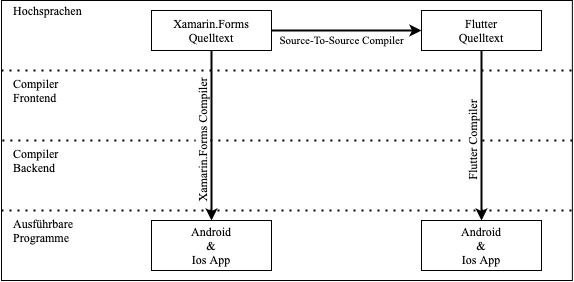
\includegraphics[width=14.5cm]{Images/CompilerArchitecture/CompilerStructure.png}
 \caption{Umfeld des Source-To-Source Compilerns}
 \label{fig:CompilerArchitecture}
\end{figure}

Die in der Abbildung skizzierten Xamarin.Forms und Flutter Compiler durchlaufen natürlich die in Kapitel 2 eingeführten Compiler-Phasen, auf dem Weg zu einer ausführbaren mobilen Anwendung.  Zusätzlich wurde in der Abbildung dargestellt,  an welcher Stelle der Source-To-Source Compiler realisiert werden soll.  Aus dieser Skizierung ist ersichtlich, dass das Ergebnis der Übersetzung, wie schon in der Definition von Source-To-Source Compilern beschrieben eine Hochsprache ist.  
Basierend auf der theoretischen Einführung von Compilern müssen bei dem Entwurf des Source to Source die Phasen aus dem Kapitel 2 betrachtet werden,  und Rückschlüssel darauf zu ziehen,  welche Arbeitsschritte in diesen Phasen durchgeführt werden müssen. Im folgenden wird anhand von Abbildung  \ref{fig:S2SCompilerAufbau} der S2- Compilers genauer betrachtet. Es ist ersichtlich,  dass sowohl Compiler-Frontend für den Übersetzer von wichtiger relvanz sind. 

\begin{figure}[!ht]
 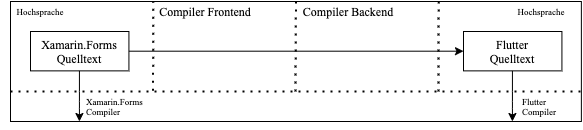
\includegraphics[width=14.5cm]{Images/CompilerArchitecture/S2SArchitecture.png}
 \caption{Source-To-Source Compiler Aufbau}
 \label{fig:S2SCompilerAufbau}
\end{figure}

Wichtig für das Ergebnis des Compilers ist es,  dass eine mit Hilfe des Xamarin.Forms Compilers Übersetzte mobile Anwendung sich identisch verhält, wie eine mit dem in dieser Arbeit realsierten S2 Compiler und dem Flutter Compiler übersetzte mobile Anwendung. 


\section{Abgrenzung}
Da es sich sowohl bei Xamarin.Forms als auch Flutter um Open-Source Frameworks handelt, welche schon seit einigen Jahren auf dem Markt sind,  hat sich  eine Vielzahl von Erweiterungen in Form von Plugins entwickelt.  Da es sich bei diesen Erweiterungen nicht zwangsläufig um Open-Source Projekte handelt hat der zu entwickelnde Übersetzer keinen Zugriff auf den Quelltext und kann diesen daher nicht Übersetzen.  Der Einfachheit halber soll der in dieser Arbeit entwickelte Prototyp ausschließlich Elemente die im Eigentlichen Framework Xamarin.Forms vorhanden sind sowie die Inhalte des Optional Verfügbaren Packetes Xamarin.Essentials, welches ebenfalls von Microsoft ist übersetzen.  Ebenfalls soll der zu implementierende Prototyp keine anderen Architekturmuster als die von Xamarin.Forms angebotenen übersetzen können.  So gibt es  Plugins wie Prism die das Model-View- ViewModel(MVVM) für Xamarin.Forms realisieren und damit dabei helfen die Geschäfts und Präsentationslogik von der Benutzeroberfläche zu trennen.  Wegen seiner Vorteile werden viele Anwendungen mithilfe von MVVM realisiert wird jedoch nicht selber von Microsoft angeboten.  Außerdem sollen der Compiler keine plattformspezifischen Lösungen übersetzt werden.
Zusammengefasst soll der zu realisierende Prototyp ausschließlich Elemente aus dem Quellframework Xamarin.Forms übersetzten, die von Micrsoft selber angeboten werden. 

Versionen

\section{Verwendung von Rosyln}
Der bereits im letzten Kapitel eingeführt Rosyln Compiler für das Übersetzen von C\# Dateien soll für den Compiler eine essentielle Rolle spielen.  Durch seinen modularen Aufbaue können die Phasen bis zur semantischen Analyse von vollständig von Roslyn durchgeführt werden.  Mithilfe des Typisierten Syntaxbaumes kann anschließend die Übersetzung zu Flutter durchgeführt werden.  

Allerdings lassen sich Xamarin.Forms Quelltext-Dokumente in zwei Kategorien unterteilen.  Den Quelltextdokumenten mit der Endung CS sowie den Dateien,  die eine Benutzeroberfläche beschreiben,  die sich nicht mit Hilfe von Roslyn übersetzen lassen.  Abbildung \ref{fig:CompilerStruktur} zeigt die Struktur des zu realisierenden Übersetzers auf einer hohen Abstraktionsebene.
\begin{figure}[!ht]
 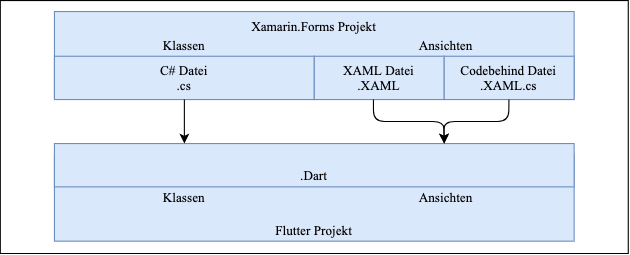
\includegraphics[width=14.5cm]{Images/Compiler/CompilerArchitecture.png}
 \caption{Compiler Struktur}
 \label{fig:CompilerStruktur}
\end{figure}




Bei den Dateien für die Ansicht handelt es sich wie in \ref{fig:CompilerStruktur} dargestellt um XAML (Extensible Application Markup Language) sowie .XAML.CS Dateien.  In einer XAML-Datei kann der Entwickler Benutzeroberflächen definieren, indem er alle Sichten, Layouts und Seiten sowie benutzerdefinierte Klassen verwendet.  Dabei hat XAML mehrere Vorteile gegenüber äquivalenten Code,  und hat sich daher in der Entwicklung von Benutzeroberflächen durchgesetzt.  So ist XAML ist prägnanter und besser lesbar als Äqivalenter Code.  Außderdem ermöglicht es die über-/unterordnungshierarchie, die in XML enthalten ist,  unterordnungshierarchie von Benutzeroberflächen Objekten zu imitieren.  Allerdings hat XAML auch den Nachteil, dass es keinen Code enthalten kann und daher immer auf Codedateien für Ereignishandler zurückgegriffen werden muss.  Diese Dateien werden häufig als .XAML.XS Dateien gespeichert und beinhalten alles was in XAML Datei nicht beinhaltet seien kann,  dazu gehören die weiter oben beschriebenen Ereignishandler,  die Events wie einen Button Knopfdruck oder die Eingabe von Text in ein Textfeld behandeln. \footcite[Vgl.][Abgerufen am \today]{MicrosoftXAML2017}
Durch eine Kombination von beiden Teilen sollte anschließend eine gleichwertige mobile Anwendung ergeben. 

\section{Code optimierung}
Die Code Optimierung ist der essentielle Teil der Übersetzung.  Beide Frameworks arbeiten grundlegend Unterschiedlich,  sodass eine einfache Übersetzung nicht zu einer funktionsfähigen Anwendung führen würde.  Daher ist es notwendig,  beide Frameworks zu analysieren und die genauen Unterschiede zwischen den Arbeitsweisen zu verstehend. Anschließend muss bei der Übersetzung darauf geachtet werden,  die Xamarin.Forms Anwendung in eine Form zu überführen bei der Sie in Form einer Flutter App auf sowohl iOS als auch Android ausgeführt werden kann.  Zu diesem Zwecke werden in dem Nachfolgenden Kapitel sowohl die Frameworks als auch die Programmiersprachen in welchen diese Entwickelt werden Analysiert um zu verstehen,  inwiefern sich Ansichten, Seiten und die Sprachen unterscheiden, und wie diese Überführt werden müssen. 

Dabei hat die Übersetzung in das Ziel Framework jedoch einen anderen Fokus,  da die Übersetzung nicht für die schnelle performance des Quelltextes verantwortlich ist, da diese Aufgabe von dem Flutter Compiler übernommen wird. 

\section{Grafische Darstellung}
